\documentclass[10pt]{beamer}

\usetheme{metropolis}
\usepackage{appendixnumberbeamer}

\usepackage{booktabs}
\usepackage[scale=2]{ccicons}

\usepackage{pgfplots}
\usepgfplotslibrary{dateplot}

\usepackage{xspace}

\usepackage{tikz}
	\usetikzlibrary{shapes.geometric, arrows, positioning}
	\tikzstyle{startstop} = [rectangle, rounded corners, minimum width=3cm, minimum 		height=1cm,text centered, draw=black, fill=red!30]
	\tikzstyle{io} = [trapezium, trapezium left angle=70, trapezium right angle=110, minimum width=3cm, minimum height=1cm, text centered, draw=black, fill=blue!30]
	\tikzstyle{process} = [rectangle, minimum width=3cm, minimum height=1cm, text centered, draw=black, fill=orange!30]
\tikzstyle{decision} = [diamond, minimum width=3cm, minimum height=1cm, text centered, draw=black, fill=green!30]
\tikzstyle{arrow} = [thick,->,>=stealth]
\tikzstyle{arrow} = [thick,->,>=stealth]
%\usepackage{listings}
\usepackage{minted}

\usepackage{bm}%................................. Bold math symbols (after fonts)

\setbeamercolor{normal text}{bg=white}





\title{EML4930/EML6934: Lecture 08}
\subtitle{Optimization with scipy.optimize }
\date{October 19, 2017}
%\author{CJ}
\author{Charles Jekel}
%\titlegraphic{\includegraphics{images/avatarCropped.png}\vspace{58cm}}
%\institute{1. University of Florida\\ 2. Stellenbosch University, South Africa}

% \titlegraphic{\hfill\includegraphics[height=1.5cm]{logo.pdf}}

\begin{document}

\maketitle

\begin{frame}{What is optimization?}
\begin{figure}
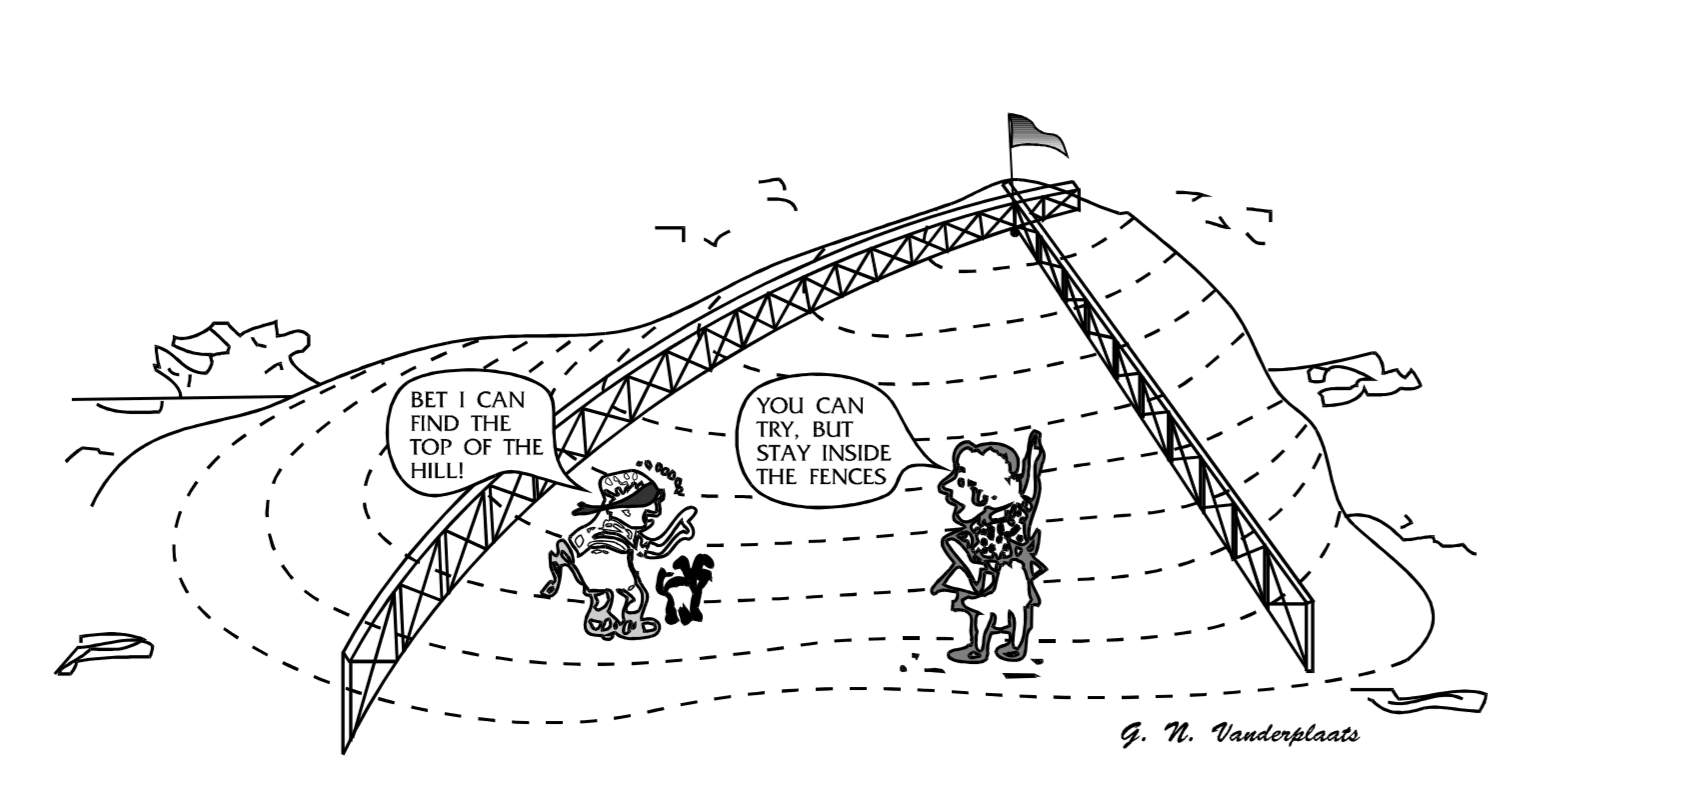
\includegraphics[width=1.0\textwidth]{figs/opt1.png}
\end{figure}

Cartoon by Dr. Gary Vanderplaats of \url{http://www.vrand.com/} some of these example problems and HW problems are from the DOT reference manual.
\end{frame}

\begin{frame}{Mathematical optimization formulation}
Objective function:
\begin{equation}
\min F(\bm{x})
\end{equation}
Inequality constraints:
\begin{equation}
G(\bm{x}) \leq 0
\end{equation}
Variable constraints
\begin{align}
x_1^L \leq x_1 \leq x_1^U \\
x_2^L \leq x_2 \leq x_2^U \\
\cdots \\
x_n^L \leq x_n \leq x_n^U 
\end{align}
\end{frame}

\begin{frame}{Optimization in engineering: finding the best input}
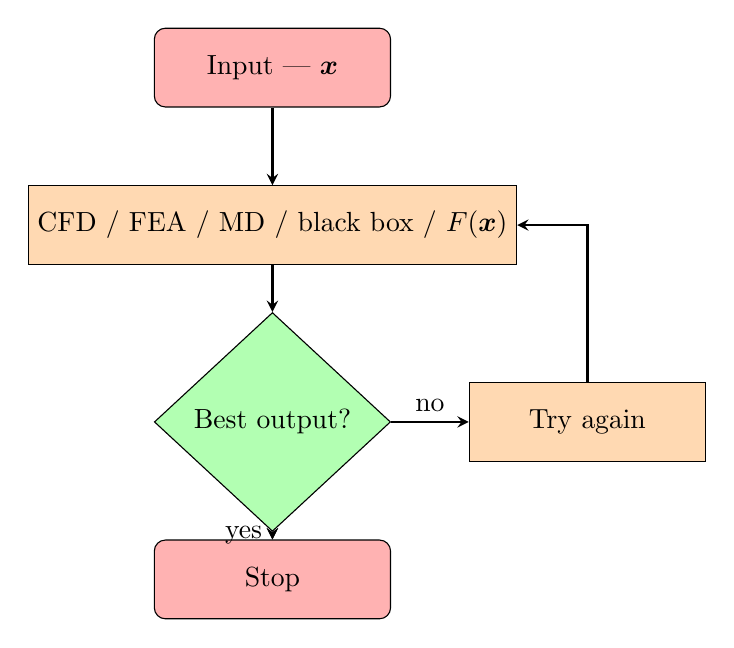
\begin{tikzpicture}[node distance=2cm]
\node (in1) [startstop] {Input | $\bm{x}$};
\node (pro1) [process, below of=in1] {CFD / FEA / MD / black box / $F(\bm{x})$};
\node (dec1) [decision, below of=pro1, yshift=-0.5cm] {Best output?};
\node (pro2b) [process, right of=dec1, xshift=2cm] {Try again};
\node (stop) [startstop, below of=dec1] {Stop};
%\draw [arrow] (start) -- (in1);
\draw [arrow] (in1) -- (pro1);
\draw [arrow] (pro1) -- (dec1);
\draw [arrow] (dec1) -- node[anchor=south] {no} (pro2b);
\draw [arrow] (pro2b) |- (pro1);
\draw [arrow] (dec1) -- node[anchor=east] {yes} (stop);
\draw [arrow] (dec1) -- (stop);
\end{tikzpicture}
\end{frame}

\begin{frame}{scipy.optimize at a glance}
\begin{itemize}
\item local and global optimization algorithms
\item gradient and stochastic
\item constrainted and unconstrained algorithms 
\end{itemize}
\url{https://docs.scipy.org/doc/scipy/reference/tutorial/optimize.html}
\url{https://docs.scipy.org/doc/scipy/reference/optimize.html}
\end{frame}

\begin{frame}{Unconstrained multivariate methods}
\begin{table}
\begin{tabular}{ll}
\textbf{Method} & \textbf{Description}  \\
\hline
fmin & Minimize a function using the downhill simplex algorithm.\\
fmin\_powell & Minimize a function using modified Powell’s method.\\
fmin\_cg & Nonlinear conjugate gradient algorithm.\\
fmin\_bfgs & Minimize a function using the BFGS algorithm.\\
fmin\_ncg &	Minimization of a function using the Newton-CG method.\\
\end{tabular}
\end{table}
\end{frame}

\begin{frame}{Constrained multivariate methods}
\begin{table}
\begin{tabular}{ll}
\textbf{Method} & \textbf{Description}  \\
\hline
fmin\_l\_bfgs\_b &	Minimize using the L-BFGS-B algorithm.\\
fmin\_tnc & 	Minimize a function with truncated Newton algorithm.\\
fmin\_cobyla &  	Constrained Optimization BY Linear Approximation.\\
fmin\_slsqp &  	Minimize using Sequential Least SQuares Programming\\
differential\_evolution & 	Finds the global minimum of a multivariate function.\\
\end{tabular}
\end{table}
\end{frame}

\begin{frame}{Global optimization methods}
\begin{table}
\begin{tabular}{ll}
\textbf{Method} & \textbf{Description}  \\
\hline
basinhopping &	Global minimum using the basin-hopping algorithm\\
brute & 	Minimize a function over a given range by brute force.\\
differential\_evolution & 	Finds the global minimum of a multivariate function.\\
\end{tabular}
\end{table}
\end{frame}

\begin{frame}{Methods I like}
\begin{table}
\begin{tabular}{lll}
\textbf{Method} & \textbf{My use} & \textbf{Pitfall}  \\
\hline
fmin\_bfgs  & local & local minima \\
fmin\_l\_bfgs\_b  & bounded local & local minima \\
fmin\_slsqp $\ast$ & Constrained local & Quadratic and local minima \\
differential\_evolution & 	Global optimization & Number of function evaluations \\
\end{tabular}
\end{table}
$\ast$ the only true constrained optimization algorithm...
\end{frame}

\begin{frame}{Optimizing engineering problems}
\begin{itemize}
\item optimization is a great design tool
\item FEA/ CFD/ MD take a long time to evaluate
\item can only afford a limited number of function evaluations
\item there is no method that will work well on all problems (see No Free Lunch by Wolpert and Macready 1997)  \url{https://ti.arc.nasa.gov/m/profile/dhw/papers/78.pdf}
\item Gradient based methods, non-gradient (stochastic) based methods, surrogate base methods, and various combinations
\end{itemize}
\end{frame}

\begin{frame}{Gradient based methods}
\begin{itemize}
\item work well when you have an initial design
\item guaranteed to find an optima (thought it might be a local one)
\item work with a large number of design variables ($ n > 1000$) 
\item make the most of your function evaluations
\item deal with multiminima by running multiple optimization from different starting point
\item function must be smooth and near continuous! 
\end{itemize}
\end{frame}

\begin{frame}{Global optimization methods}
\begin{itemize}
\item large number of function evaluations (which is fine when you can afford it)
\item stochastic/evolutionary methods not guaranteed to converge to a minima
\item sometimes we just want to find the best solution
\item functions can be discontinuous 
\end{itemize}
\end{frame} 

\begin{frame}[fragile]{fmin\_bfgs basic gradient based method}
\url{https://docs.scipy.org/doc/scipy/reference/generated/scipy.optimize.fmin_bfgs.html#scipy.optimize.fmin_bfgs}
\begin{minted}
{python}
res = fmin_bfgs(f, x0, fprime=None, args=(), gtol=1e-05, 
norm=inf, epsilon=1.4901161193847656e-08, maxiter=None, 
full_output=0,  disp=1, retall=0, callback=None)
\end{minted}
\end{frame}

\begin{frame}[fragile]{fmin\_l\_bfgs\_b constrained version of BFGS}
\url{https://docs.scipy.org/doc/scipy/reference/generated/scipy.optimize.fmin_l_bfgs_b.html#scipy.optimize.fmin_l_bfgs_b}
\begin{minted}
{python}
res = fmin_l_bfgs_b(func, x0, fprime=None, args=(), 
approx_grad=0, bounds=None, m=10, factr=10000000.0, 
pgtol=1e-05, epsilon=1e-08,  iprint=-1, maxfun=15000, 
maxiter=15000, disp=None,   callback=None, maxls=20)
\end{minted}
\end{frame}

\begin{frame}[fragile]{differential evolution}
\url{https://docs.scipy.org/doc/scipy/reference/generated/scipy.optimize.differential_evolution.html#scipy.optimize.differential_evolution}
\begin{minted}
{python}
res = differential_evolution(func, bounds, args=(), 
strategy='best1bin', maxiter=1000, popsize=15, tol=0.01,
 mutation=(0.5, 1), recombination=0.7,  seed=None, 
 callback=None,  disp=False, polish=True,   
 init='latinhypercube', atol=0)
\end{minted}
\end{frame}

\begin{frame}{differential evolution parameters}
I really love all the feature with this algorithm... 
\begin{itemize}
\item strategy: the differential evolution strategy
\item polish: if true a L-BFGS-B optimization is run with the optima found by differential evolution (This is a true meta-heuristic algorithm! - great global optimization) 
\item init: by default the first generation is made with a latin hypercube sampling!
\end{itemize}
warning this could use a considerable number of function evaluations
\end{frame}

\begin{frame}{Example 1: non-linear regression with BFGS 1 of 3}
Consider fitting a function
\begin{equation}
f(\bm{\beta}, x) = \frac{\beta_0 x}{\beta_1 + x}
\end{equation}
in this case $\bm{\beta}$ are the design variables and x are the data points. 

For this example I'm going to fit this function to some data points. 

In most cases you won't know the exact beta parameters that the data comes from, but it makes for an easy example to know the solution.

\end{frame}

\begin{frame}[fragile]{Example 1: non-linear regression with BFGS 2 of 3}
\begin{minted}
{python}
import numpy as np
import matplotlib.pyplot as plt
from scipy import optimize

# generate some data from known beta values
x = np.linspace(0,10,30)
beta0 = 2.7
beta1 = 1.3
y = (beta0*x)/(beta1+x)

# determine beta by minimizing the mean residual error
def my_func(X):
    yHat = (X[0]*x)/(X[1]+x)
    resid = yHat - y
    return np.mean(np.abs(resid))
\end{minted}
\end{frame}

\begin{frame}[fragile]{Example 1: non-linear regression with BFGS 3 of 3}
\begin{minted}
{python}
# peform the optimization with bfgs
x0 = [3.0, 3.0] # initial guess
res = optimize.fmin_bfgs(my_func, x0, full_output=True) 

plt.figure()
plt.plot(x,y,'o')
beta = res[0] # these are the resulting beta parameters
# plot the resulting curve
plt.plot(x,(beta[0]*x)/(beta[1]+x))
plt.show()
\end{minted}
\end{frame}

\begin{frame}[fragile]{Example 2: constrained optimization 1 of 4}
Minimize
\begin{equation}
F(\bm{x}) = (x_0 + x_1)^2 + (x_1 + x_2)^2
\end{equation}
subject to
\begin{equation}
h_0 = x_0 + 2x_1 + 3x_2 - 1 = 0
\end{equation}
from the initial design point of
\begin{equation}
\bm{x_0} = [-4.0, 1.0, 2.0]
\end{equation}
\textbf{Note}: You always set up your equality constraints equal to 0!
\end{frame}

\begin{frame}[fragile]{Example 2: constrained optimization 2 of 4}
\begin{minted}
{python}
# objective function
def func(X):
    F = (X[0]+X[1])**2 + (X[1]+X[2])**2
    return F
# equality constraint
def f_con(X):
    G = X[0] + 2.0*X[1] + 3.0*X[2] - 1.0
    return G
# initial design point
x0 = np.array([-4.0, 1.0, 2.0])    
res = optimize.fmin_slsqp(func, x0, f_eqcons=f_con,
    iter=1000, acc=1e-06, disp=True, full_output=True)
\end{minted}
\end{frame}

\begin{frame}[fragile]{Example 2: constrained optimization 3 of 4}
Minimize
\begin{equation}
F(\bm{x}) = (x_0 + x_1)^2 + (x_1 + x_2)^2
\end{equation}
subject to an alternative inequality constraints
\begin{equation}
g_0 = x_0 + 2x_1 + 3x_2 - 1 \leq 0
\end{equation}
\begin{equation}
g_1 = -g_0 \leq 0
\end{equation}
from the initial design point of
\begin{equation}
\bm{x_0} = [-4.0, 1.0, 2.0]
\end{equation}
\textbf{Note}: You always set up your inequality constraints less than or equal to zero!
\end{frame}

\begin{frame}[fragile]{Example 2: constrained optimization 4 of 4}
\begin{minted}
{python}
# objective function
def func(X):
    F = (X[0]+X[1])**2 + (X[1]+X[2])**2
    return F
# inequality constraint
# note slsqp handles Gradient contraints as >= 0 and not <=0
# so for this case i have G >= 0 and -G > = 0
# don't ask me why... I have no clue why
def f_con1(X):
    G = X[0] + 2.0*X[1] + 3.0*X[2] - 1.0
    return G, -G
# initial design point
x0 = np.array([-4.0, 1.0, 2.0])    
res = optimize.fmin_slsqp(func, x0, f_ieqcons=f_con1, 
    iter=1000, acc=1e-06, disp=True, full_output=True)
\end{minted}
\end{frame}

\begin{frame}{Example 3: Global optimization of the Adjiman function}
Minimize
\begin{equation}
f( \bm{x} ) = \cos (x_0) \sin (x_1) - \frac{x_0}{x_1^2 +1}
\end{equation}
on the domain
\begin{equation}
-10 \leq x_0 \leq 10
\end{equation}
\begin{equation}
-10 \leq x_1 \leq 10
\end{equation}
\end{frame}

\begin{frame}[fragile]{Example 3: Global optimization of the Adjiman function}
Differential evolution works well on this multimodal problem.
\begin{minted}
{python}
# objective function
def adjiman(x):
    F = np.cos(x[0])*np.sin(x[1]) - ((x[0])/(x[1]**2 +1.0))
    return F
    
# optimization bounds 
bounds = ((-10.0,10.0),
          (-10.0,10.0))    
# run differential evolution          
res = optimize.differential_evolution(adjiman, bounds, 
    maxiter=1000, popsize=50, disp=True)
\end{minted}
\end{frame}

\begin{frame}{Example 3: Global optimization of the Adjiman function}
\begin{figure}
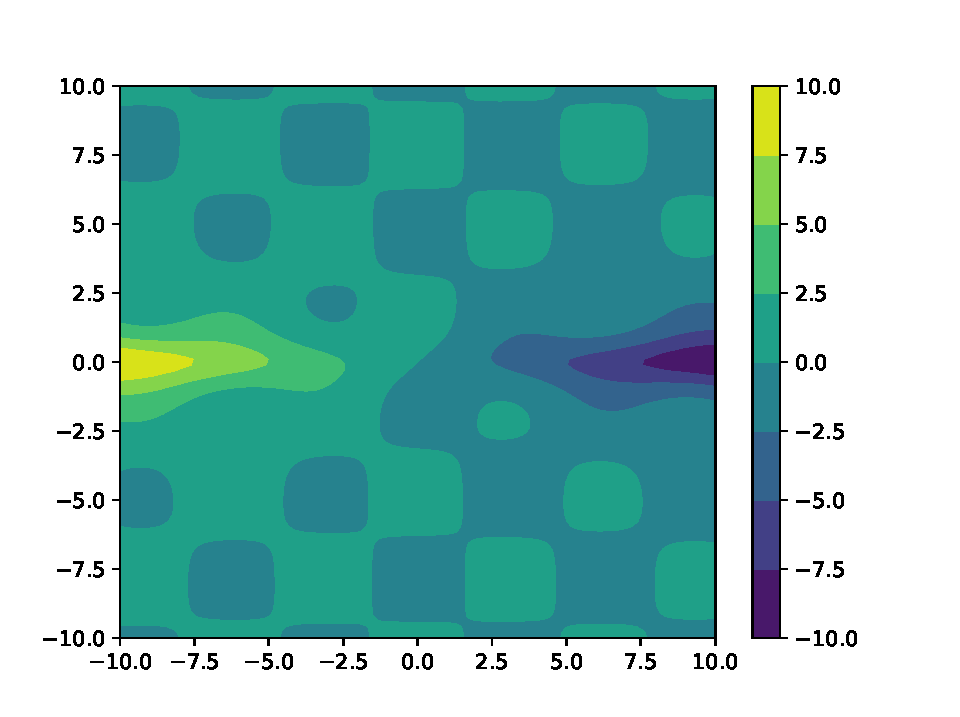
\includegraphics[width=1.0\textwidth]{figs/adjiman.pdf}
\end{figure}
\end{frame}

\begin{frame}[fragile]{Example 3: Global optimization of the Adjiman function}
Issues with L-BFGS-B
\begin{minted}
{python}
# objective function
def adjiman(x):
    F = np.cos(x[0])*np.sin(x[1]) - ((x[0])/(x[1]**2 +1.0))
    return F
    
# optimization bounds 
bounds = ((-10.0,10.0),
          (-10.0,10.0))    
          
# this l bfgs b won't find the optimum
res2 = optimize.fmin_l_bfgs_b(adjiman, (-2,-2), 
    approx_grad=True, bounds=bounds)

# however this l bfgs b will
res3 = optimize.fmin_l_bfgs_b(adjiman, (2,2), 
    approx_grad=True, bounds=bounds)
\end{minted}
\end{frame}


%\begin{frame}{Supplementary textbook for statistics in Python}
%Freely available.
%
%Think Stats by Allen B. Downey.
%Exploratory Data Analysis in Python.
%
%\url{http://greenteapress.com/wp/think-stats-2e/}
%\end{frame}
%
%\begin{frame}{Statistics with scipy.stats}
%
%Today we're going to discuss many features of scipy.stats
%
%The full documentation is available:
%\url{https://docs.scipy.org/doc/scipy/reference/stats.html}
%
%Part of this lecture will cover the tutorial here:
%\url{https://docs.scipy.org/doc/scipy/reference/tutorial/stats.html}
%\end{frame}
%
%\begin{frame}{What will we cover today}
%\begin{itemize}
%\item Random variable distributions
%\item Continuous and discrete distributions
%\item PDF, CDF, SF, and other associated functions of distributions
%\item Maximum likelihood estimation to fit distributions to data
%\item Hypothesis test: are two samples from the same distribution?
%\item Hypothesis test: are these samples from this distribution?
%\end{itemize}
%\end{frame}
%
%\begin{frame}[fragile]{Reminder of viewing documentation}
%In Python the documentation is included with the library.
%\begin{minted}
%{python}
%from scipy import stats
%# documentation of the namespace one screen at a time
%stats?
%# print the entire documentation
%print(stats.__doc__)
%# Don't forget the help function
%help(stats)
%# for a particular function
%stats.norm?
%# or
%print(stats.norm.__doc__)
%# __doc__ is a built in attribute created from the 
%# comments following your function definition!
%# view all of the contents in scipy.stats
%dir(stats)
%\end{minted}
%\end{frame}
%
%\begin{frame}{scipy.stats at a glance}
%\begin{itemize}
%\item 95 continuous distributions
%\item 13 discrete distributions
%\item 9 multivariate distributions
%\item A number of other statistical functions and methods
%\end{itemize}
%\end{frame}
%
%\begin{frame}{Common methods for continuous random variable distributions}
%\begin{table}
%\begin{tabular}{ll}
%\textbf{Method} & \textbf{Description}  \\
%\hline
%    rvs & Random Variates \\
%    pdf & Probability Density Function \\
%    cdf & Cumulative Distribution Function \\
%    sf & Survival Function (1-CDF) \\
%    ppf & Percent Point Function (Inverse of CDF) \\
%    isf & Inverse Survival Function (Inverse of SF)  \\
%    stats & Return mean, variance, (Fisher’s) skew, or (Fisher’s) kurtosis \\
%    moment & non-central moments of the distribution \\
%\end{tabular}
%\end{table}
%\end{frame}
%
%\begin{frame}[fragile]{scipy.stats namespace}
%\begin{minted}
%{python}
%from scipy import stats
%
%# the namespace follows:
%# scipy.stats.distribution.method()
%
%# demonstrating how to access methods of the 
%# Maxwell continuous distribution
%stats.maxwell.rvs()
%stats.maxwell.pdf(1)
%stats.maxwell.cdf(1)
%stats.maxwell.sf(1)
%stats.maxwell.ppf(0.5)
%
%\end{minted}
%\end{frame}
%
%\begin{frame}[fragile]{It's safe to import the distributions themselves}
%If you're only going to use a few functions and distributions, it may make sense to import them directly.
%\begin{minted}
%{python}
%from scipy.stats import norm
%from scipy.stats import binom
%from scipy.stats import poisson
%
%# now we can call the distributions directly
%norm.pdf(0.9)
%
%binom.cdf(8,n=100,p=0.1)
%
%poisson.rvs(1)
%\end{minted}
%\end{frame}
%
%\begin{frame}{Basic methods take vectorized input}
%Basic methods such as pdf, and cdf are vectorized with np.vectorize.
%
%
%pdf(0.5) will calculate the pdf at 0.5
%
%
%cdf(0.5) will calculate the cdf at 0.5
%
%
%However often we want to calculate the pdf and cdf at more than one value. For these cases we pass a numpy array of values into the functions.
%
%
%pdf(x) will return an array of the same shape x of the pdf value of each item in x
%
%
%\end{frame}
%
%\begin{frame}[fragile]{Let's take a look at the normal distribution}
%\mint{python}|scipy.stats.norm|
% scipy.stats.\_continuous\_distns.norm\_gen object
% A normal continuous random variable.
%
%The location (loc) keyword specifies the mean. The scale (scale) keyword specifies the standard deviation.
%
%\begin{minted}
%{python}
%import matplotlib.pyplot as plt
%x = np.linspace(-3,3,100)
%# the default normal distribution has a mean of 0
%# and standard deviation of 1
%y = norm.pdf(x)
%plt.figure()
%plt.plot(x,y)
%plt.show()
%\end{minted}
%\end{frame}
%
%\begin{frame}[fragile]{We can specify the mean and standard deviation}
%\begin{minted}
%{python}
%mu = 2.0
%std = 2.0
%x = np.linspace(-4.0,8.0,100)
%y = norm.pdf(x, mu, std)
%z = norm.cdf(x, mu, std)
%w = norm.sf(x, mu, std)
%
%# plot the pdf, cdf, and sf
%plt.figure()
%plt.plot(x,y)
%plt.plot(x,z)
%plt.plot(x,w)
%plt.show()
%\end{minted}
%\end{frame}
%
%\begin{frame}{Digression: Meaning of PDF, CDF, and SF}
%These are for continuous random variable $x$.
%\smallskip
%\smallskip
%
%PDF - probability density function
%
%PDF tells you the probability of a particular random variate occurring.
%P($x = 0.5$) = PDF(0.5)
%
%\smallskip
%\smallskip
%
%CDF - cumulative distribution function
%
%CDF tells you the probability of a particular random variate being less than or equal to a value.
%
%P($-\infty < t \leq m $) = CDF($m$) = $\int_{-\infty}^{m} PDF(t) dt$
%
%P($ -\infty < x\leq 0.5$) = CDF(0.5)
%\smallskip
%\smallskip
%
%
%SF - survival function
%
%SF tells you the probability of a particular random variate being greater than a value.
%
%P($x > 0.5$) = SF(0.5) = 1 - CDF(0.5)
%\smallskip
%\smallskip
%\end{frame}
%
%\begin{frame}[fragile]{Back to the normal distribution}
%It's tedious to always specify the $mu, \sigma$ for each function. So what we do is create a \textit{Frozen} instance of the object. You won't be able to change the $mu, \sigma$ of the \textit{Frozen} instance.
%
%\begin{minted}
%{python}
%mu1 = 2.0; std1 = 2.0
%mu2 = 3.0; std2 = 1.0
%
%# create a frozen normal distribution object
%# from mu1, std1
%my_norm1 = norm(mu1,std1)
%
%# create a second frozen normal distribution object
%my_norm2 = norm(mu2,std2)
%\end{minted}
%\end{frame}
%
%\begin{frame}[fragile]{Working with a \textit{Frozen} instance}
%\begin{minted}
%{python}
%# you'll see this will have all of the functions of norm
%print(dir(my_norm1))
%
%# let's plot the pdf of my_norm1 and my_norm2
%x = np.linspace(-4.0,8.0,100)
%plt.figure()
%plt.plot(x, my_norm1.pdf(x))
%plt.plot(x, my_norm2.pdf(x))
%plt.show()
%\end{minted}
%\end{frame}
%
%\begin{frame}[fragile]{Working with a \textit{Frozen} instance: generating random variables}
%We can use the \textit{rvs} method to generate samples of random variables. The random generation relies on numpy's pseudorandom number generator. This means we can seed the random number generator to ensure the result is reproducible. 
%
%\begin{minted}
%{python}
%# seed the random number generator
%np.random.seed(1012301)
%
%# generate 100 samples from my_norm1
%rv1 = my_norm1.rvs(100)
%# generate 10000 samples from my_norm2
%rv2 = my_norm2.rvs(10000)
%
%\end{minted}
%\end{frame}
%
%\begin{frame}[fragile]{Compare the histogram of the generated samples to the pdf}
%\begin{minted}
%{python}
%# plot the histogram of the random samples and compare 
%# to the pdf values
%
%plt.figure()
%plt.hist(rv1, normed=True)
%plt.hist(rv2, bins=30, normed=True)
%plt.plot(x, my_norm1.pdf(x))
%plt.plot(x, my_norm2.pdf(x))
%plt.show()
%\end{minted}
%\end{frame}
%
%\begin{frame}[fragile]{Compare cumulative distribution of samples to the cdf}
%\begin{minted}
%{python}
%# plot the cumulative histogram of the samples 
%# and compare with the true cdf 
%
%plt.figure()
%plt.hist(rv1, cumulative=True, normed=True)
%plt.hist(rv2, bins=30, cumulative=True, normed=True)
%plt.plot(x, my_norm1.cdf(x))
%plt.plot(x, my_norm2.cdf(x))
%plt.show()
%\end{minted}
%\end{frame}
%
%\begin{frame}[fragile]{What does the following code do?}
%Does this code generate 10 samples from the normal distribution? 
%\mint{python}|norm.rvs(10)|
%... \textbf{Be careful!}
%\end{frame}
%
%\begin{frame}[fragile]{Be explicit by providing specifying the keywords}
%Use the \textit{size} keyword to specify the number of samples to generate from a distribution.
%
%The following code will produce the same random samples
%\begin{minted}
%{python}
%np.random.seed(82)
%aa = norm.rvs(10,3,1000)
%
%np.random.seed(82)
%bb = norm.rvs(loc=10, scale=3, size=1000)
%# is aa exactly equal to bb?
%print((aa == bb).all())
%
%# if you specify the keywords, you can change the order
%np.random.seed(82)
%cc = norm.rvs(size=1000, loc=10, scale=3) 
%# is cc exactly equal to bb?
%print((cc == bb).all())
%\end{minted}
%\end{frame}
%
%\begin{frame}[fragile]{Continuous distributions in general}
%Use \textit{loc} and \textit{scale} to shift and scale distributions. However some distributions require additional shape parameters. To view the number of additional shape parameters use
%\mint{python}|distrubituion_name.numargs|
%
%Some examples:
%\begin{minted}
%{python}
%in : print(stats.norm.numargs)
%out: 0
%
%in : print(stats.gamma.numargs)
%out: 1
%
%in : print(stats.beta.numargs)
%out: 2
%\end{minted}
%\textbf{Note}: there is not a shape keyword.
%\end{frame}
%
%\begin{frame}[fragile]{How do you figure out how to specify the shape parameters?}
%\mint{python}|stats.beta?|
%\begin{figure}
%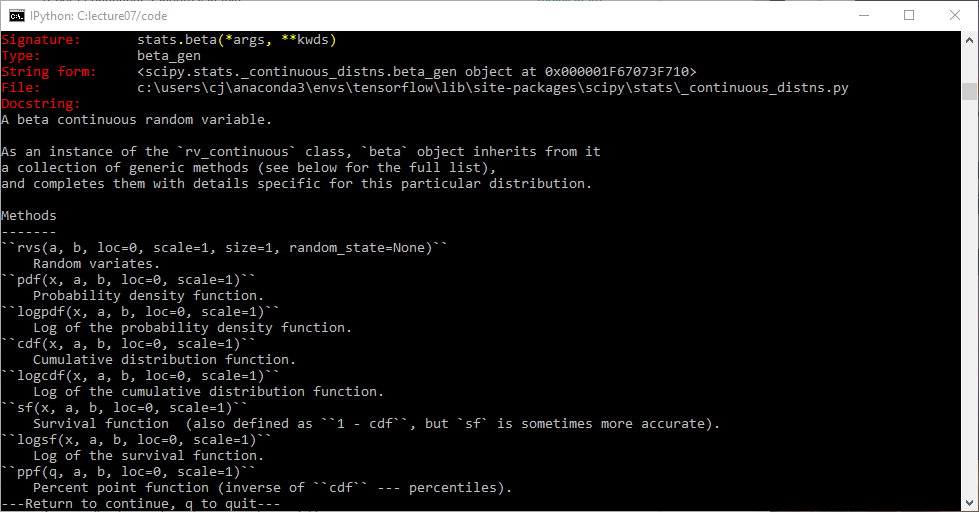
\includegraphics[width=1.0\textwidth]{figs/betaDist.png}
%\end{figure}
%The shape parameters for the beta random variate distribution are $a$ and $b$. In this case the order of the shape parameters matters!
%\end{frame}
%
%\begin{frame}{Methods for fitting distributions}
%You most often use \textit{fit} to perform a maximum likelihood estimation of a distribution's parameters. Maximum likelihood estimations (MLE) can be very ill-posed, so it's recommended to provide \textit{fit} with a reasonable starting point.
%\begin{table}
%\begin{tabular}{ll}
%\textbf{Method} & \textbf{Description}  \\
%\hline
%    fit & maximum likelihood estimation of parameters\\
%    fit\_loc\_scale & estimation of loc and scale provided shape parameters\\
%    nnlf & negative log likelihood function\\
%    expect & Calculate the expectation of a function against the pdf or pmf\\
%\end{tabular}
%\end{table}
%\textbf{Note}: these methods aren't available for every distribution
%\end{frame}
%
%\begin{frame}{From the tutorial: Performance issues and cautionary remarks}
%\begin{itemize}
%\item the performance of each distribution is different
%\item some methods within distributions are explicitly calculated (by evaluating an analytic expression)
%\item others are calculated with more costly methods if there is no analytically form (ie using generic algorithms)
%\item MLE isn't a good choice for some distributions
%\end{itemize}
%\end{frame}
%
%\begin{frame}[fragile]{You can build your own distributions using Subclassing}
%Making a continuous distribution is simple and many values will be computed automatically.
%\begin{minted}
%{python}
%from scipy import stats
%class deterministic_gen(stats.rv_continuous):
%    def _cdf(self, x):
%        return np.where(x < 0, 0., 1.)
%    def _stats(self):
%        return 0., 0., 0., 0.
%\end{minted}
%\end{frame}
%
%\begin{frame}{Whats different with discrete distributions?}
%\begin{itemize}
%\item Discrete distributions don't have a pdf, however they do have a pmf (probability mass function)
%\item No estimation methods such as \textit{fit}
%\item \textit{scale} is not valid, but \textit{loc} still is
%\item cdf is a step function, thus inverse cdf (ppf) works a little bit differently
%\begin{equation}
%\text{ppf}(q) = \min (x: \text{cdf} (x) \geq q, x \text{integer}) 
%\end{equation}
%\end{itemize}
%\end{frame}
%
%\begin{frame}[fragile]{Enter the binomial distribution}
%\begin{minted}
%{python}
%from scipy.stats import binom
%# binom requires two arguments, n and p
%n = 100   # number of trials
%p = 1./6. # probability that you win
%
%my_binom = binom(n,p)
%
%n_wins = np.arange(0,40,1)
%plt.figure()
%plt.plot(n_wins,my_binom.pmf(n_wins), 'o')
%plt.show()
%
%# what is the proability that you'll win at least 16 times?
%print(my_binom.sf(15))
%
%# what is the probability that you won't win more than 25 times? 
%print(my_binom.cdf(24))
%\end{minted}
%\end{frame}
%
%\begin{frame}[fragile]{Example: fitting a distribution 1 of 3}
%\begin{minted}
%{python}
%# let's generate random samples from a normal distribution
%# and fit a beta distribution to the samples
%
%np.random.seed(467)
%rv = norm.rvs(loc=4.0,scale=1.0,size=10000)
%
%# estimate the mean and variance
%est_loc = np.mean(rv)
%est_scale = np.std(rv)
%
%# perform the MLE to determine the beta parameters
%beta_param = stats.beta.fit(rv, loc=est_loc, scale=est_scale)
%
%# create the beta model
%beta_fit = stats.beta(*beta_param)
%# equiv to stats.beta(beta_param[0], beta_param[1], ...
%\end{minted}
%\end{frame}
%
%\begin{frame}[fragile]{Example: fitting a distribution 2 of 3}
%\begin{minted}
%{python}
%# let's compare the pdf from the fitted beta distribution
%# to the histogram of the samples
%
%x = np.linspace(1.0, 7.0, 100)
%
%plt.figure()
%plt.hist(rv, bins=30, normed=True)
%plt.plot(x, beta_fit.pdf(x))
%plt.show()
%
%# and the cdf to the cumulative histogram
%plt.figure()
%plt.hist(rv, bins=30, cumulative=True, normed=True)
%plt.plot(x, beta_fit.cdf(x))
%plt.show()
%\end{minted}
%\end{frame}
%
%\begin{frame}[fragile]{Example: fitting a distribution 3 of 3}
%\begin{minted}
%{python}
%# we can use the Kolmogorov-Smirnov test to perform a 
%# hypothesis test to see if our samples do come from beta
%
%# Hypothesis: the rv does indeed come from beta distribution
%# for 99% confidence reject if pvalue is less than 0.01
%
%test_res = stats.kstest(rv, 'beta', beta_param)
%print('KS-statistic D = %6.3f pvalue = %6.4f' % test_res )
%
%# is this better than a ufitted normal estimate?
%test_norm = stats.kstest(rv, 'norm', (np.mean(rv), np.std(rv)))
%print('KS-statistic D = %6.3f pvalue = %6.4f' % test_norm )
%\end{minted}
%\textbf{Note}: Dont' use pvalues to deice if anything is quantitative better than anything else! The pvalue is just an accept or reject of the hypothesis. 
%\end{frame}
%
%\begin{frame}[fragile]{Kolmogorov-Smirnov test for two sample}
%This is a hypothesis test for to determine whether two sets of samples originate from the same distribution. 
%
%Hypotheses: The samples come from the same distribution.
%Reject if he hypothesis when the pvalue is small.
%\begin{minted}
%{python}
%np.random.seed(1212)
%rvs1 = stats.norm.rvs(loc=5, scale=10, size=500)
%rvs2 = stats.norm.rvs(loc=5, scale=10, size=100)
%rvs3 = stats.norm.rvs(loc=4, scale=14, size=200)
%
%# test wheter 1 and 2 come from the same distribution
%# for 95% confidece we reject if the pvalue is less than 0.05
%
%test_12 = stats.ks_2samp(rvs1, rvs2)
%test_13 = stats.ks_2samp(rvs1, rvs3)
%test_23 = stats.ks_2samp(rvs2, rvs3)
%
%\end{minted}
%\end{frame}
%
%\begin{frame}{So what did we cover today}
%\begin{itemize}
%\item Introduction to statistics with scipy.stats
%\item How the object oriented frozen distributions work
%\item Random variable distributions
%\item Continuous and discrete distributions
%\item PDF, CDF, SF, and other associated functions of distributions
%\item Maximum likelihood estimation to fit distributions to data
%\item Hypothesis test: are two samples from the same distribution?
%\item Hypothesis test: are these samples from this distribution?
%\end{itemize}
%\end{frame}
%
%\begin{frame}{So whats still out there?}
%\begin{itemize}
%\item There is a lot more that we can't cover in one day...
%\item We can make an entire class on statistics in Python
%\item We didn't cover multivariate distributions...
%\item There are numerous other functions in scipy.stats
%\item There are plotting tools in scipy.stats (probability plots, box plots, etc.)
%\end{itemize}
%\end{frame}



\end{document}
